\documentclass{beamer}
\mode<presentation>
\usepackage{amsmath}
\usepackage{amssymb}
\usepackage{algorithmic}
%\usepackage{advdate}
\usepackage{adjustbox}
\usepackage{subcaption}
\usepackage{enumitem}
\usepackage{multicol}
\usepackage{mathtools}
\usepackage{listings}
\usepackage{url}
\def\UrlBreaks{\do\/\do-}
\usetheme{Boadilla}
\usecolortheme{lily}
\setbeamertemplate{footline}
{
	\leavevmode%
	\hbox{%
		\begin{beamercolorbox}[wd=\paperwidth,ht=2.25ex,dp=1ex,right]{author in head/foot}%
			\insertframenumber{} / \inserttotalframenumber\hspace*{2ex} 
	\end{beamercolorbox}}%
	\vskip0pt%
}
\setbeamertemplate{navigation symbols}{}

\providecommand{\nCr}[2]{\,^{#1}C_{#2}} % nCr
\providecommand{\nPr}[2]{\,^{#1}P_{#2}} % nPr
\providecommand{\mbf}{\mathbf}
\providecommand{\pr}[1]{\ensuremath{\Pr\left(#1\right)}}
\providecommand{\qfunc}[1]{\ensuremath{Q\left(#1\right)}}
\providecommand{\sbrak}[1]{\ensuremath{{}\left[#1\right]}}
\providecommand{\lsbrak}[1]{\ensuremath{{}\left[#1\right.}}
\providecommand{\rsbrak}[1]{\ensuremath{{}\left.#1\right]}}
\providecommand{\brak}[1]{\ensuremath{\left(#1\right)}}
\providecommand{\lbrak}[1]{\ensuremath{\left(#1\right.}}
\providecommand{\rbrak}[1]{\ensuremath{\left.#1\right)}}
\providecommand{\cbrak}[1]{\ensuremath{\left\{#1\right\}}}
\providecommand{\lcbrak}[1]{\ensuremath{\left\{#1\right.}}
\providecommand{\rcbrak}[1]{\ensuremath{\left.#1\right\}}}
\theoremstyle{remark}
\newtheorem{rem}{Remark}
\newcommand{\sgn}{\mathop{\mathrm{sgn}}}
\providecommand{\abs}[1]{\left\vert#1\right\vert}
\providecommand{\res}[1]{\Res\displaylimits_{#1}} 
\providecommand{\norm}[1]{\lVert#1\rVert}
\providecommand{\mtx}[1]{\mathbf{#1}}
\providecommand{\mean}[1]{E\left[ #1 \right]}
\providecommand{\fourier}{\overset{\mathcal{F}}{ \rightleftharpoons}}
%\providecommand{\hilbert}{\overset{\mathcal{H}}{ \rightleftharpoons}}
\providecommand{\system}{\overset{\mathcal{H}}{ \longleftrightarrow}}
%\newcommand{\solution}[2]{\textbf{Solution:}{#1}}
%\newcommand{\solution}{\noindent \textbf{Solution: }}
\providecommand{\dec}[2]{\ensuremath{\overset{#1}{\underset{#2}{\gtrless}}}}
\newcommand{\myvec}[1]{\ensuremath{\begin{pmatrix}#1\end{pmatrix}}}
\let\vec\mathbf

\lstset{
	%language=C,
	frame=single, 
	% breaklines=true,
	columns=fullflexible
}

\numberwithin{equation}{section}

\title{Identify and Solve a Quadratic Equation}
\author{Eshan Sharma - EE24BTECH11022}

\date{\today} 
\begin{document}
	
	\begin{frame}
		\titlepage
	\end{frame}
	
	\section*{Outline}
	\begin{frame}
		\tableofcontents
	\end{frame}
	
	\section{Problem}
	\begin{frame}
		\frametitle{Problem Statement}
		A pole has to be erected at a point on the boundary of a circular park of diameter 13 metres in such a way that the difference of its distances from two diametrically opposite fixed gates A and B on the boundary is 7 metres. Is it possible to do so? If yes, at what distances from the two gates should the pole be erected?
	\end{frame}
	
	%\subsection{Literature}
	\section{Solution}
	
	\subsection{Quadratic Equation}
	\begin{frame}
		\frametitle{Quadratic Equation}
		
		Let the distance of the pole from gate B be \(x\) metres. Then the distance from gate A will be \((x+7)\) metres.
		
		From the Pythagoras theorem, since \(\triangle APB\) is a right triangle:
		\begin{align}
			AB^2 = AP^2 + BP^2
		\end{align}
		Given \(AB = 13\) metres, substituting values:
		\begin{align}
			13^2 &= (x+7)^2 + x^2 \\
			169 &= x^2 + 14x + 49 + x^2 \\
			2x^2 + 14x - 120 &= 0
		\end{align}
		Simplify the equation:
		\begin{align}
			x^2 + 7x - 60 &= 0
		\end{align}
	\end{frame}
	
	\subsection{Theoretical Solution}
	\begin{frame}
		\frametitle{Theoretical Solution}
		Using the quadratic formula \(x = \frac{-b \pm \sqrt{b^2 - 4ac}}{2a}\), where \(a = 1, b = 7, c = -60\):
		\begin{align}
			x &= \frac{-7 \pm \sqrt{7^2 - 4(1)(-60)}}{2(1)} \\
			x &= \frac{-7 \pm \sqrt{289}}{2} \\
			x &= \frac{-7 \pm 17}{2}
		\end{align}
		Thus, \(x = 5\) or \(x = -12\). Since distance cannot be negative, \(x = 5\).
		The distances are:\
		\(BP = 5\) metres, \(AP = 12\) metres.
		
	\end{frame}

	
	\subsection{Computational Newton's Method}
	\begin{frame}[allowframebreaks]
		\frametitle{Computational Newton's Method}
		Newton's method formula is:
		\begin{align}
			x_{n+1} = x_n - \frac{f(x_n)}{f'(x_n)}
		\end{align}
		Define \(f(x) = x^2 + 7x - 60\) and \(f'(x) = 2x + 7\). The iterative formula becomes:
		\begin{align}
			x_{n+1} = x_n - \frac{x_n^2 + 7x_n - 60}{2x_n + 7}
		\end{align}
		Starting with an initial guess \(x_0 = 0\):
		\begin{align}
			x_1 &= 5 \quad \text{(converges to 5)}
		\end{align}
		Thus, \(x = 5\) is the root.\\
		
		\begin{figure}[h]
			\centering
			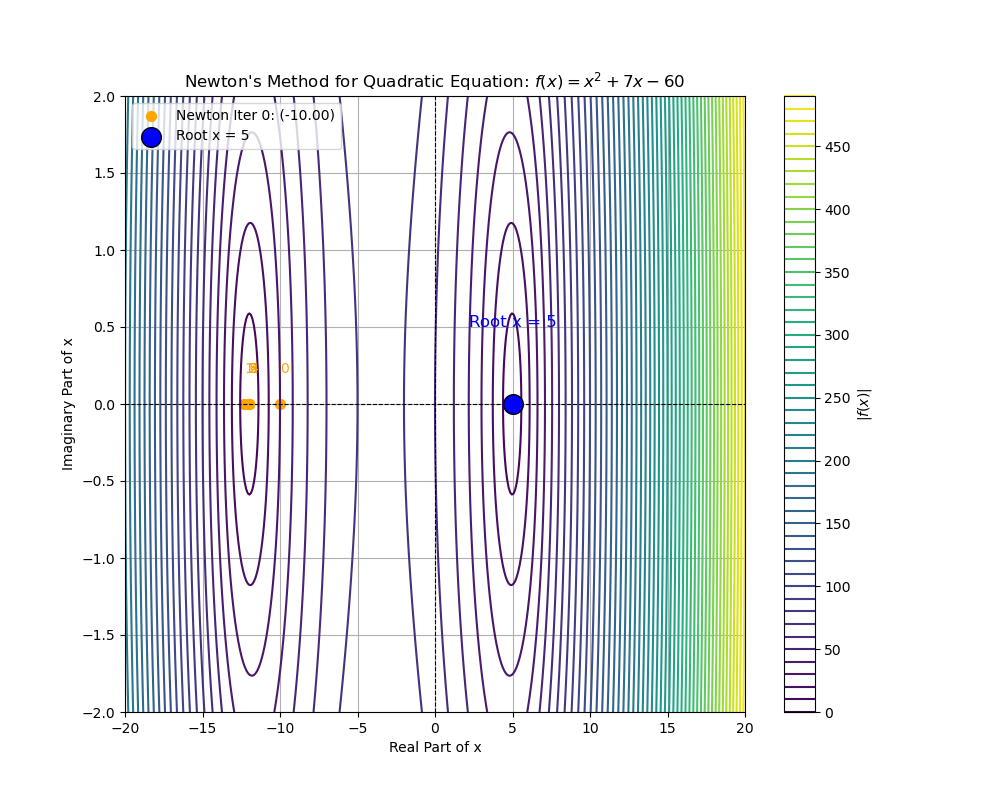
\includegraphics[width=0.8\textwidth]{fig2.png}
		\end{figure}
		
	\end{frame}
	
	
	\subsection{Companion Matrix}
	\begin{frame}[allowframebreaks]
		\frametitle{Companion Matrix}
		
		We are given the quadratic equation \(x^2 + 7x - 60 = 0\) and need to solve it using the QR decomposition method. The companion matrix is:
		\[
		A_0 = \begin{bmatrix} 0 & -60 \\ 1 & -7 \end{bmatrix}
		\]
		
		Step 1: QR Decomposition of \(A_0\)
		The QR decomposition of \(A_0\) is:
		\[
		Q_0 = \begin{bmatrix} 0 & 1 \\ 1 & 0 \end{bmatrix}, \quad
		R_0 = \begin{bmatrix} 1 & -7 \\ 0 & 60 \end{bmatrix}
		\]
		
		Step 2: Update \(A_1\)
		Now, we update \(A_1 = R_0 Q_0\):
		\[
		A_1 = \begin{bmatrix} -7 & 60 \\ 60 & 0 \end{bmatrix}
		\]
		
		Step 3: QR Decomposition of \(A_1\)
		Next, we compute the QR decomposition of \(A_1\):
		\[
		Q_1 = \begin{bmatrix} -0.116 & 0.993 \\ 0.993 & 0.116 \end{bmatrix}, \quad
		R_1 = \begin{bmatrix} -60.57 & 6.93 \\ 0 & 60.28 \end{bmatrix}
		\]
		
		Step 4: Update \(A_2\)
		We update \(A_2 = R_1 Q_1\):
		\[
		A_2 = \begin{bmatrix} -6.93 & 60.28 \\ 60.28 & 0.57 \end{bmatrix}
		\]
		
		Step 5: Convergence
		Continuing the iterations, we eventually reach the matrix:
		\[
		T = \begin{bmatrix} 5 & 0 \\ 0 & -12 \end{bmatrix}
		\]
		The eigenvalues of \(T\) are \( \lambda_1 = 5 \) and \( \lambda_2 = -12 \), which are the roots of the quadratic equation.
		
		Thus, the solutions to the equation \(x^2 + 7x - 60 = 0\) are:
		\[
		x = 5 \quad \text{and} \quad x = -12
		\]
		
	\end{frame}

	\subsection{Plotting the curve}
	\begin{frame}
		\frametitle{Plotting the curve}
		\begin{figure}[h]
			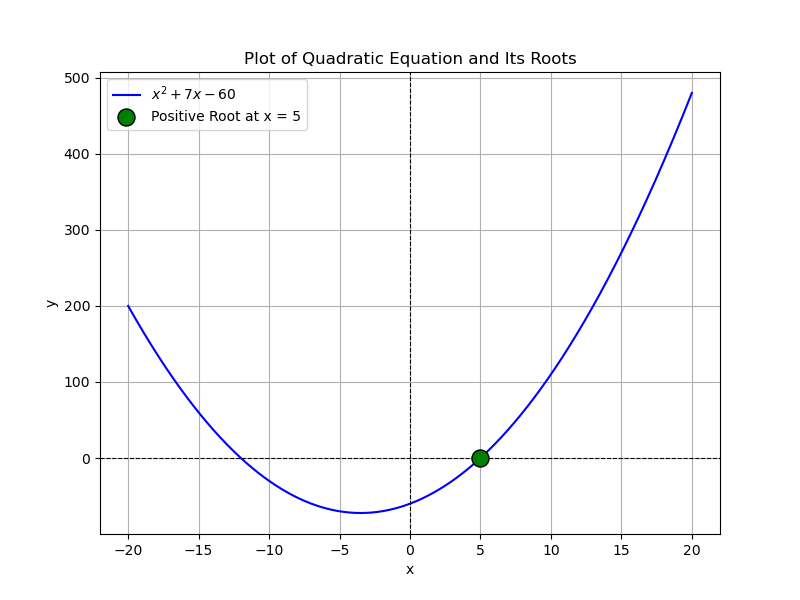
\includegraphics[scale=0.5]{fig.png}
			\centering
		\end{figure}
	\end{frame}
	
\end{document}